% Borrador para IEEE Transactions on Instrumentation and Measurement (IEEEtran, journal).
% Figuras y tablas: generadas por recon/articulo.py (./run.sh articulo). Numeros del texto: datos/numeros.json.
\documentclass[journal]{IEEEtran}
\usepackage[T1]{fontenc}
\usepackage{amsmath,amssymb}
\usepackage{graphicx}
\usepackage{booktabs,multirow}
\usepackage[table]{xcolor}
\usepackage{cite}
\usepackage{url}
\usepackage{tikz}
\usetikzlibrary{arrows.meta,positioning,fit,calc}
\newcommand{\printmae}{0.13}
\newcommand{\printrms}{0.21}
\newcommand{\printmax}{0.5}
\newcommand{\nobj}{5}
\newcommand{\nerfR}{1.64}
\newcommand{\nerfS}{1.32}
\newcommand{\nerfD}{+0.32}
\newcommand{\nerfFR}{0.79}
\newcommand{\nerfFS}{0.85}
\newcommand{\nerfICP}{1.62}
\newcommand{\nerfshift}{0.3}
\newcommand{\gsR}{2.06}
\newcommand{\gsS}{2.00}
\newcommand{\gsD}{+0.06}
\newcommand{\gsFR}{0.70}
\newcommand{\gsFS}{0.75}
\newcommand{\gsICP}{2.06}
\newcommand{\gsshift}{0.5}
\newcommand{\mvsR}{2.10}
\newcommand{\mvsS}{2.13}
\newcommand{\mvsD}{-0.02}
\newcommand{\mvsFR}{0.73}
\newcommand{\mvsFS}{0.73}
\newcommand{\mvsICP}{2.04}
\newcommand{\mvsshift}{0.7}
\newcommand{\rgbdR}{4.01}
\newcommand{\rgbdS}{0.40}
\newcommand{\rgbdD}{+3.61}
\newcommand{\rgbdFR}{0.37}
\newcommand{\rgbdFS}{0.98}
\newcommand{\rgbdICP}{3.02}
\newcommand{\rgbdshift}{7.2}

\newcommand{\todo}[1]{\textcolor{red}{[TODO: #1]}}

\begin{document}

\title{Quantifying the Sim-to-Real Gap of 3D Reconstruction With Paired Real and Digital-Twin Captures}

\author{Juan Ulises Calderon Huerta, Jonathan Daniel Navarrete Gomez,
        and Dora Luz Almanza Ojeda,~\IEEEmembership{Member,~IEEE}%
\thanks{Manuscript received \todo{date}. \todo{Affiliations and funding.}}}

\markboth{IEEE Transactions on Instrumentation and Measurement,~Vol.~XX, No.~X, 2026}%
{Shell \MakeLowercase{\textit{et al.}}: Sim-to-Real Gap of 3D Reconstruction}

\maketitle

\begin{abstract}
Simulated captures are increasingly used to develop and validate 3D reconstruction pipelines, but how far
their accuracy transfers to physical measurements has not been quantified for the main families of methods.
We present a paired benchmark in which each real capture of a 3D-printed object, acquired with three fixed
Intel RealSense L515 cameras and a ChArUco-instrumented turntable, is reproduced in NVIDIA Isaac Sim with
the same camera intrinsics, extrinsics and per-stop turntable poses. Both captures are processed with four
techniques---neural radiance fields (NeRF), 3D Gaussian splatting (3DGS), multi-view stereo (MVS) and
RGB-D TSDF fusion---using identical inputs and known poses, and every cloud is cleaned and scored with the
same protocol against the CAD model: accuracy, completeness, Chamfer distance, 95th-percentile Hausdorff
distance and F-score at 1, 2 and 5~mm. The twin reproduces the real board detections with a median
reprojection difference of \textbf{0.11~px} and object silhouettes with IoU~$\geq$~\textbf{0.975}, and the
printing error of the reference artifact, measured with a caliper, is \textbf{\printmae~mm} MAE. For the
image-based methods the twin predicts the real Chamfer distance within a few tenths of a millimeter on
average, whereas RGB-D fusion---the most accurate method in simulation (\textbf{\rgbdS~mm})---is the least
accurate on real data (\textbf{\rgbdR~mm}), dominated by a 5--16~mm offset of the L515 depth with respect
to the photogrammetric frame. We release the capture format, the twin, and the evaluation code.
\end{abstract}

\begin{IEEEkeywords}
3D reconstruction, digital twin, sim-to-real gap, neural radiance fields, Gaussian splatting, multi-view
stereo, RGB-D sensors, LiDAR camera, metrology, measurement uncertainty.
\end{IEEEkeywords}

% ============================================================================================
\section{Introduction}
\IEEEPARstart{D}{ense} 3D reconstruction from images and depth is a measurement problem: a physical surface
is estimated from noisy observations, and its fitness for inspection, robotic grasping or digital-twin
construction depends on a quantifiable error. Four families dominate current practice. Multi-view stereo
(MVS) \cite{schoenberger2016sfm,schoenberger2016mvs} triangulates photo-consistent pixels; neural radiance
fields (NeRF) \cite{mildenhall2020nerf,mueller2022instant} and 3D Gaussian splatting (3DGS)
\cite{kerbl2023gaussian} optimize a radiance representation from which depth can be rendered; and RGB-D
fusion integrates active depth maps into a truncated signed distance function (TSDF)
\cite{curless1996volumetric,newcombe2011kinectfusion}.

Comparative studies of these methods are numerous but fragmented
\cite{remondino2023critical,zielinski2026comparative,arshad2024plant,rs2025archaeo,isprs2025gs}: they
usually cover two or three families, are performed on real data only, and take as reference a laser or
structured-light scan whose own error is of the same order as the quantity being measured. At the same
time, photorealistic simulators such as NVIDIA Isaac Sim \cite{isaacsim} make it cheap to generate captures
with exact ground truth, and are increasingly used to develop and tune reconstruction pipelines. Whether an
error measured in simulation predicts the error of the same pipeline on the physical object---the
\emph{sim-to-real gap of the reconstruction itself}---has, to the best of our knowledge, not been quantified
across these four families. Existing sim-to-real studies measure the gap on downstream tasks such as object
detection \cite{sudhakar2023sim2real} or manipulation \cite{qureshi2024splatsim}, and the closest
metrological precedent, VIRTUS-FPP \cite{haroon2026virtus}, pairs a physical and a simulated
fringe-projection sensor for a single technique and object.

This paper contributes:
\begin{enumerate}
\item A \emph{paired} real/digital-twin acquisition: every real turntable capture is reproduced in Isaac Sim
with the measured intrinsics, rig extrinsics and per-stop board poses, and the fidelity of the twin is
itself measured (fiducial reprojection and silhouette agreement).
\item A single evaluation protocol for NeRF, 3DGS, MVS and RGB-D fusion that uses identical inputs and known
poses, a reproducible cloud-cleaning procedure, and a consensus 4-DOF registration of the CAD model to the
real reconstructions.
\item A traceable reference: 3D-printed objects whose CAD model is the ground truth in both domains, with
the CAD-to-print deviation measured independently.
\item Per-method, per-object quantification of the sim-to-real gap over five objects and seven metrics,
which identifies depth-to-color registration of the active sensor, rather than reconstruction itself, as
the dominant real-world error source of RGB-D fusion.
\end{enumerate}

% ============================================================================================
\section{Related Work}
\subsection{Comparative evaluation of reconstruction techniques}
Remondino \emph{et al.} \cite{remondino2023critical} compared seven NeRF variants with COLMAP MVS against
scanner references and found that NeRF outperforms MVS on non-cooperative (texture-less, reflective,
transparent) surfaces, while MVS wins on well-textured ones. NeRFBK \cite{karami2023nerfbk} provides a
benchmark with high-accuracy scans and Blender-rendered objects. Zieli\'nski \emph{et al.}
\cite{zielinski2026comparative} evaluated COLMAP, 3DGS, 2DGS and several NeRF variants on YCB objects with
precision, recall and F-score at 2 and 5~mm, and showed that the ranking depends on the metric; although
they recorded RGB-D data, depth fusion was not evaluated. Similar comparisons exist for plants
\cite{arshad2024plant}, archaeological artifacts \cite{rs2025archaeo}, real-world scenes \cite{isprs2025gs},
and terrestrial laser scanning \cite{jutzi2023tls}. Classical benchmarks such as DTU \cite{jensen2014dtu} and
Tanks and Temples \cite{knapitsch2017tanks} established accuracy/completeness and F-score as standard
metrics, which we adopt.

\subsection{Reference geometry and 3D-printed artifacts}
Reference geometry is typically obtained with structured-light or laser scanners
\cite{remondino2023critical,jutzi2023tls}, whose uncertainty adds to the measured error. 3D-printed objects
with known CAD models have been used as stable references for plant phenotyping \cite{boemer2024plant}, for
image-to-CAD reconstruction under domain shift \cite{realcad2026}, and for comparing photogrammetry with
structured light \cite{sensors2025industrial}; additive-manufacturing metrology registers scans of printed
parts to their CAD to quantify dimensional deviations \cite{jms2020printed}. We follow this approach and
measure the CAD-to-print deviation of our reference artifact directly.

\subsection{Simulation, digital twins and the sim-to-real gap}
Digital-twin datasets pair real objects with high-fidelity models \cite{dong2025dtc,kuang2023orb}, and
Sudhakar \emph{et al.} \cite{sudhakar2023sim2real} matched real and synthetic captures of YCB objects to
study the gap in object detection. Gaussian-splatting simulators \cite{qureshi2024splatsim,robogsim2024}
use reconstruction as a tool to \emph{close} the gap for robot learning, and Isaac Sim is used to generate
repeatable RGB-D data \cite{bonetto2023grade}; however, simulated depth is usually ideal
\cite{realitygap2025}. The closest work, VIRTUS-FPP \cite{haroon2026virtus}, builds a virtual
fringe-projection profilometer in Isaac Sim and its physical counterpart, scans a printed figurine and
compares both against the STL, reporting sub-millimeter real--virtual differences. Our study generalizes
this design to four passive and active reconstruction families, five objects and a complete set of
point-cloud metrics.

% ============================================================================================
\section{Measurement System and Digital Twin}
\begin{figure*}[!t]
\centering
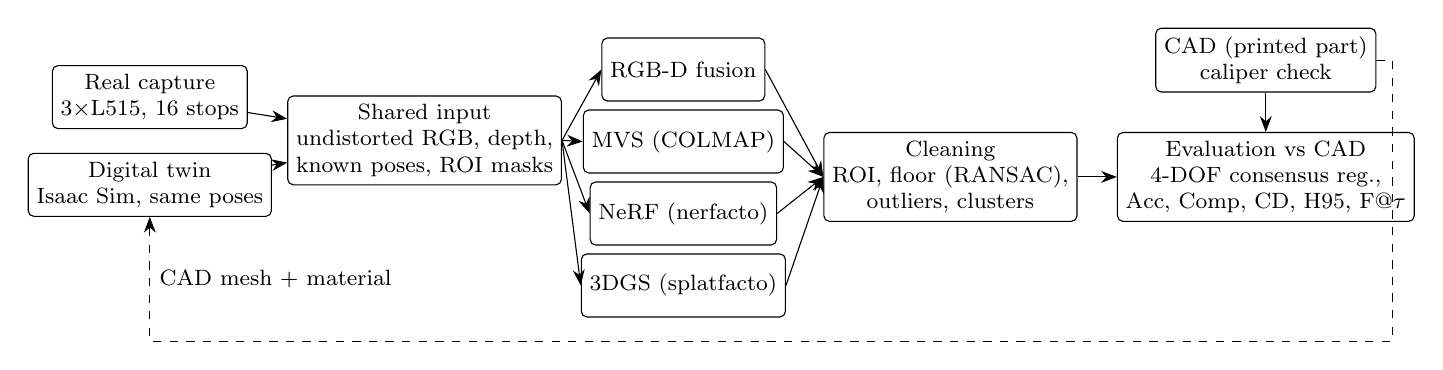
\begin{tikzpicture}[node distance=3mm and 5mm, font=\footnotesize,
  box/.style={draw, rounded corners=2pt, align=center, minimum height=8mm, inner sep=3pt, fill=white},
  arr/.style={-{Stealth[length=2mm]}}]
\node[box] (real) {Real capture\\3$\times$L515, 16 stops};
\node[box, below=of real] (twin) {Digital twin\\Isaac Sim, same poses};
\node[box, right=of real, yshift=-5.5mm] (in) {Shared input\\undistorted RGB, depth,\\known poses, ROI masks};
\node[box, right=of in, yshift=9mm] (m1) {RGB-D fusion};
\node[box, below=1mm of m1] (m2) {MVS (COLMAP)};
\node[box, below=1mm of m2] (m3) {NeRF (nerfacto)};
\node[box, below=1mm of m3] (m4) {3DGS (splatfacto)};
\node[box, right=of m2, yshift=-4.5mm] (cl) {Cleaning\\ROI, floor (RANSAC),\\outliers, clusters};
\node[box, right=of cl] (ev) {Evaluation vs CAD\\4-DOF consensus reg.,\\Acc, Comp, CD, H95, F@$\tau$};
\node[box, above=of ev, yshift=2mm] (cad) {CAD (printed part)\\caliper check};
\draw[arr] (real) -- (in); \draw[arr] (twin) -- (in);
\foreach \m in {m1,m2,m3,m4} {\draw[arr] (in.east) -- (\m.west); \draw[arr] (\m.east) -- (cl.west);}
\draw[arr] (cl) -- (ev); \draw[arr] (cad) -- (ev);
\draw[arr, dashed] (cad.east) -- ++(2mm,0) |- ($(m4.south)+(0,-3mm)$) -| node[pos=0.75, right]{CAD mesh + material} (twin.south);
\end{tikzpicture}
\caption{Overview of the paired benchmark. The same pipeline processes the real capture and its digital
twin; only the source of the images and depth maps differs.}
\label{fig:pipeline}
\end{figure*}

\subsection{Acquisition rig}
Three Intel RealSense L515 LiDAR cameras \cite{intel2020l515} (\emph{high}, \emph{middle}, \emph{low}) are
fixed around a turntable that carries the object on a ChArUco board (10$\times$7 squares of 24~mm, 18~mm
markers, DICT\_5X5\_250 \cite{garrido2014aruco}) printed on a letter-size sheet. A capture consists of 16
stops per revolution; at each stop every camera records one 1280$\times$720 color image and ten depth frames
(0.25~mm depth units). The pose of the board in each color camera is detected with OpenCV~4.10 and fused
across cameras in a common rig frame (the color frame of the reference camera), so every view has a
metric pose in the board frame. The resulting 48 views per capture are the input to all methods.

\subsection{Digital twin}
The twin is built in Isaac Sim~6.2 with the RTX renderer. Cameras are placed with the real rig extrinsics
and remain fixed; the turntable assembly (sheet, cardboard and object) is rotated at each stop by the
measured board transform, so the final camera-to-board poses reproduce the real ones exactly. The OpenCV
pinhole model with the real intrinsics is used for the color lens, with a half-pixel correction of the
principal point because the RTX pinhole schema places the pixel origin at the corner. The object is the CAD
mesh (millimeters, Z-up) placed at a canonical pose---bounding box centered on the turntable axis, yaw
zero, resting on the board---with a material matched to the filament (Table~\ref{tab:capturas}). The real
objects were placed by hand, so their pose on the board, recovered afterwards by the CAD registration of
Section~\ref{sec:registro}, differs from the canonical one: by a rotation of about 180$^\circ$ (Bunny-S,
PI2, P1) or 90$^\circ$ (Caesar), and by a 37~mm offset from the axis at zero yaw (Bunny-L). Because the
16 stops are spaced by 22.5$^\circ$, a 90$^\circ$ or 180$^\circ$ rotation leaves the set of object-relative
viewpoints unchanged up to a cyclic shift of the stops; what differs is the direction of the static
lighting relative to the object and, for Bunny-L, the distance to the cameras. Depth maps are rendered ideally and degraded with a provisional
sensor model: zero-mean Gaussian noise with a per-camera standard deviation (3.5, 1.6 and 0.9~mm for the
high, middle and low cameras), 6\% random dropout and invalidation of pixels at depth discontinuities larger
than 20~mm. The twin is written in exactly the real capture format, so the reconstruction code cannot
distinguish both sources.

\subsection{Twin fidelity}
The fidelity of each twin is measured before reconstruction (Table~\ref{tab:capturas}). First, the ChArUco
board is detected in every rendered view with the same OpenCV version and its corners are compared with
the projection of the board under the real pose; the median difference is 0.106--0.117~px. Second, the
rendered object silhouette is compared with the projection of the CAD mesh at its twin pose through the
real cameras; the median
intersection-over-union is 0.975--0.989, with centroid offsets below 0.25~px. These values bound the
geometric disagreement between both domains that is due to the twin itself.

\begin{table}[!t]
\centering\footnotesize
\caption{Test objects (CAD size), filament, and fidelity of the digital twin: median ChArUco reprojection
difference and median silhouette IoU over the 48 views.}
\label{tab:capturas}
\begin{tabular}{lcccc}
\toprule
Object & Size (mm) & Material & Reproj. (px) & IoU \\
\midrule
Bunny-S & 86$\times$67$\times$83 & PLA beige & 0.117 & 0.975 \\
Bunny-L & 173$\times$134$\times$166 & PLA beige & 0.107 & 0.977 \\
PI2 & 140$\times$100$\times$48 & PLA beige & 0.115 & 0.986 \\
P1 & 100$\times$70$\times$33 & PETG grey & 0.113 & 0.981 \\
Caesar & 122$\times$135$\times$200 & PLA glow (transl.) & 0.106 & 0.989 \\
\bottomrule
\end{tabular}

\end{table}

\begin{figure*}[!t]
\centering
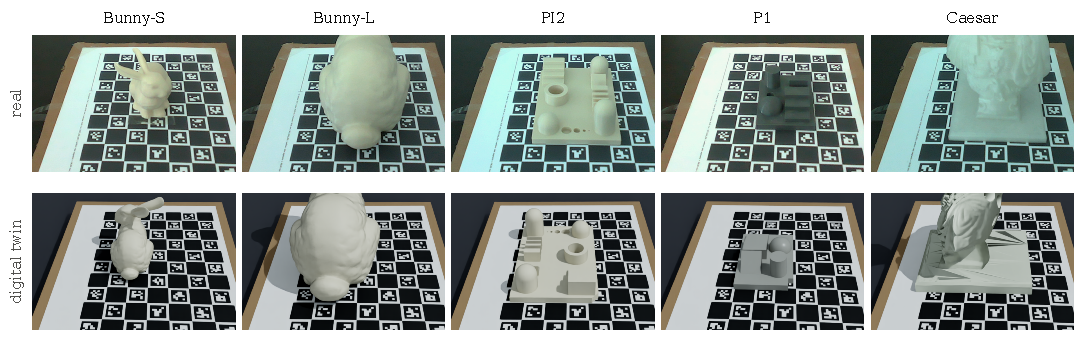
\includegraphics[width=\textwidth]{figuras/gemelo.pdf}
\caption{Real captures (top) and their digital twins (bottom), middle camera, first stop. Camera and board
poses are identical; the twin object is placed at a canonical pose (centered on the axis, yaw zero), whereas
the real one was placed by hand (rotated about 180$^\circ$ for Bunny-S, PI2 and P1, 90$^\circ$ for Caesar,
37~mm off-axis for Bunny-L). Material and lighting are approximated.}
\label{fig:gemelo}
\end{figure*}

\subsection{Test objects and printing accuracy}
Five FDM-printed objects were captured (Fig.~\ref{fig:gemelo}): the Stanford bunny at two scales (Bunny-S,
Bunny-L), a bust of Caesar printed in a translucent glow-in-the-dark PLA, and two metrological artifacts
with primitive features (PI2 and P1). Because the CAD model, not the printed part, is used as ground truth,
the CAD-to-print deviation is an error floor for every method. It was measured on P1 with a caliper
(resolution 0.1~mm) on 15 features (Table~\ref{tab:impresion}). The external dimensions match the CAD
exactly; the deviations follow known FDM effects: first-layer squish (+0.3~mm in base height), wall
over-extrusion (+0.2~mm), rounding of a sharp 45$^\circ$ edge ($-0.3$~mm) and an undersized bore
($-0.5$~mm). The mean absolute deviation is \printmae~mm (RMS \printrms~mm, maximum \printmax~mm), an order
of magnitude below the reconstruction errors reported below.

\begin{table}[!t]
\centering\footnotesize
\caption{CAD-to-print deviation of the P1 artifact (caliper, 0.1~mm resolution).}
\label{tab:impresion}
\begin{tabular}{lrrr}
\toprule
Feature & CAD (mm) & Printed (mm) & $\Delta$ (mm) \\
\midrule
Base length & 100.0 & 100.0 & +0.0 \\
Base width & 70.0 & 70.0 & +0.0 \\
Base height & 8.0 & 8.3 & +0.3 \\
Step height 1 & 13.0 & 13.0 & +0.0 \\
Step height 2 & 18.0 & 18.0 & +0.0 \\
Step height 3 & 23.0 & 23.0 & +0.0 \\
Step width & 16.0 & 16.2 & +0.2 \\
Step depth & 30.0 & 30.2 & +0.2 \\
Cylinder diameter & 20.0 & 20.0 & +0.0 \\
Cylinder height & 33.0 & 33.4 & +0.4 \\
Dome height & 23.0 & 23.1 & +0.1 \\
Ramp height & 28.0 & 27.7 & -0.3 \\
Bore diameter & 10.0 & 9.5 & -0.5 \\
Notch length & 12.0 & 12.0 & +0.0 \\
Notch width & 6.0 & 6.0 & +0.0 \\
\midrule
\multicolumn{3}{l}{MAE / RMS / max $|\Delta|$ (n = 15)} & 0.13 / 0.21 / 0.5 \\
\bottomrule
\end{tabular}

\end{table}

% ============================================================================================
\section{Reconstruction Methods}
All methods receive the same input: undistorted color images (pinhole model), the known camera poses in the
board frame, region-of-interest (ROI) masks given by a vertical cylinder around the turntable axis, and, for
RGB-D fusion, the depth frames. Poses are never re-estimated, so the comparison isolates surface
reconstruction from pose estimation. All outputs are expressed in the board frame in meters.

\emph{RGB-D fusion.} For each view, pixels valid in at least half of the ten frames are averaged and
back-projected through the depth intrinsics and the depth-to-color extrinsics of each L515. The 48 clouds
are refined by multi-view point-to-plane ICP \cite{besl1992icp} with a Tukey kernel (2~mm) between
neighboring stops and cameras (corrections limited to 5~mm), and integrated in a TSDF
\cite{curless1996volumetric} with 1.5~mm voxels and 6~mm truncation (Open3D \cite{zhou2018open3d}).

\emph{MVS.} COLMAP \cite{schoenberger2016sfm,schoenberger2016mvs} triangulates a sparse model with the fixed
poses and runs patch-match stereo with geometric consistency at full resolution; depth maps are fused with
a minimum of three consistent pixels inside the ROI masks.

\emph{NeRF.} Nerfacto \cite{tancik2023nerfstudio} is trained for 30\,000 iterations with camera optimization
disabled. Expected depth is rendered for every training view (pixels with accumulated opacity $\geq 0.5$)
and fused in the same TSDF as above.

\emph{3DGS.} Splatfacto (gsplat \cite{ye2024gsplat}) is initialized from the triangulated sparse points and
trained for 30\,000 iterations; rendered depth is fused in the same TSDF.

Each fused surface is sampled with 300\,000 points to obtain the evaluated cloud.

% ============================================================================================
\section{Evaluation Protocol}
\subsection{Point-cloud cleaning}
Every cloud, real or synthetic, is cleaned with the same parameters before scoring
(Fig.~\ref{fig:limpieza}):
\begin{enumerate}
\item \emph{ROI}: points outside the cylinder around the turntable axis are removed.
\item \emph{Floor}: the board plane is fitted by RANSAC \cite{fischler1981ransac} (1.5~mm threshold) in the
outer ring of the ROI ($r > 0.75R$), which never contains the object. The 99th percentile of the height of
that ring measures the apparent thickness of the reconstructed floor, which is large for NeRF and 3DGS; points
below $\max(5~\text{mm}, \text{thickness} + 1~\text{mm})$ are removed.
\item \emph{Statistical outliers} ($k = 20$ neighbors, $2\sigma$).
\item \emph{Floating clusters}: DBSCAN \cite{ester1996dbscan} ($\varepsilon = 4$~mm) on a 1.5~mm voxel grid;
the seed is the largest cluster that touches the floor (the object rests on the board), and other large
clusters within 15~mm of it are kept. The contact condition prevents a sheet of 3DGS floaters, larger than a
small object, from being selected.
\end{enumerate}

\begin{figure}[!t]
\centering
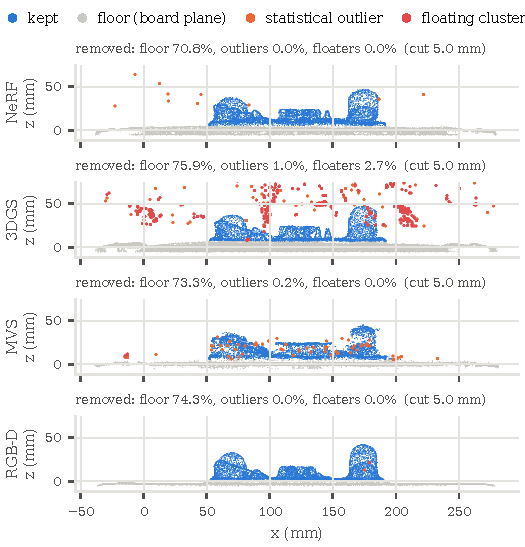
\includegraphics[width=\columnwidth]{figuras/limpieza.pdf}
\caption{Cleaning of the real PI2 reconstructions (side view). Floaters above the plotted range are
counted in the titles.}
\label{fig:limpieza}
\end{figure}

\subsection{Ground-truth registration}\label{sec:registro}
In the twin, the CAD pose is known. In the real capture, the object position on the board is not, so the
CAD mesh is registered to the reconstructions with a 4-DOF ICP (translation and yaw; the object rests on
the board and cannot tilt): a yaw sweep in 15$^\circ$ steps followed by ICP at 15, 5 and 2~mm, solving the
yaw and translation in closed form (2D Procrustes \cite{umeyama1991}) with a vertical offset. The
registration is computed on each method's cleaned cloud, and the pose with the lowest median (over methods)
of the median cloud-to-mesh distance is used for \emph{all} methods (consensus pose). A per-method ICP is
reported separately to separate shape error from placement error.

\subsection{Metrics}
The CAD mesh is cropped at the floor-cut height of each method, because the band near the base is neither
observable nor kept, and sampled with 300\,000 points. Let $\mathcal{P}$ be the reconstructed cloud and
$\mathcal{G}$ the GT samples. \emph{Accuracy} is the distance from each $p\in\mathcal{P}$ to the mesh and
\emph{completeness} the distance from each $g\in\mathcal{G}$ to $\mathcal{P}$; we report their medians. The
Chamfer distance (CD) is the average of their means, and H95 is the 95th percentile of the symmetric
distances. For a threshold $\tau$, precision $P(\tau)$ and recall $R(\tau)$ are the fractions of accuracy and
completeness distances below $\tau$, and $F(\tau) = 2PR/(P+R)$, reported at 1, 2 and 5~mm
\cite{knapitsch2017tanks}. All metrics are computed without ICP (shape + placement in the board frame);
the sim-to-real gap is $\Delta = m_\text{real} - m_\text{twin}$.

% ============================================================================================
\section{Results}
% Seccion de resultados. Numeros de tablas/numeros.tex (generados); los citados por objeto vienen de
% tablas/resultados.tex: revisarlos si se re-evalua.
\begin{table*}[!t]
\centering
\caption{Per-object results without ICP. R = real capture, T = digital twin, $\Delta$ = R $-$ T. CD: Chamfer
distance; Acc./Comp.: median accuracy/completeness; F@$\tau$: F-score at $\tau$~mm; H95: 95th-percentile
Hausdorff distance. Bold: best method for that object, domain and metric.}
\label{tab:resultados}
\resizebox{\textwidth}{!}{\scriptsize\begin{tabular}{llrrrrrrrrrrrrrrrr}
\toprule
& & \multicolumn{3}{c}{CD (mm) $\downarrow$} & \multicolumn{2}{c}{Acc. (mm) $\downarrow$} & \multicolumn{2}{c}{Comp. (mm) $\downarrow$} & \multicolumn{2}{c}{F@1 $\uparrow$} & \multicolumn{3}{c}{F@2 $\uparrow$} & \multicolumn{2}{c}{F@5 $\uparrow$} & \multicolumn{2}{c}{H95 (mm) $\downarrow$} \\
\cmidrule(lr){3-5} \cmidrule(lr){6-7} \cmidrule(lr){8-9} \cmidrule(lr){10-11} \cmidrule(lr){12-14} \cmidrule(lr){15-16} \cmidrule(lr){17-18}
Object & Method & R & T & $\Delta$ & R & T & R & T & R & T & R & T & $\Delta$ & R & T & R & T \\
\midrule
\multirow{4}{*}{Bunny-S} & NeRF & \textbf{0.87} & 0.72 & +0.15 & \textbf{0.57} & 0.51 & \textbf{0.68} & 0.59 & \textbf{0.77} & 0.86 & \textbf{0.93} & 0.97 & -0.04 & 0.99 & 0.99 & 3.1 & 2.1 \\
 & 3DGS & 0.97 & 1.32 & -0.35 & 0.71 & 0.79 & 0.82 & 0.84 & 0.65 & 0.63 & 0.92 & 0.86 & +0.06 & \textbf{0.99} & 0.96 & \textbf{2.8} & 6.7 \\
 & MVS & 1.24 & 1.30 & -0.06 & 0.75 & 0.73 & 0.99 & 0.90 & 0.56 & 0.58 & 0.84 & 0.82 & +0.02 & 0.98 & 0.97 & 4.3 & 5.6 \\
 & RGB-D & 3.07 & \textbf{0.29} & +2.78 & 2.30 & \textbf{0.14} & 3.08 & \textbf{0.33} & 0.18 & \textbf{0.98} & 0.38 & \textbf{1.00} & -0.62 & 0.86 & \textbf{1.00} & 9.8 & \textbf{0.7} \\
\midrule
\multirow{4}{*}{Bunny-L} & NeRF & \textbf{1.73} & 1.70 & +0.03 & 1.08 & 0.90 & \textbf{1.00} & 0.86 & 0.48 & 0.57 & \textbf{0.79} & 0.82 & -0.03 & \textbf{0.93} & 0.93 & 9.4 & 9.3 \\
 & 3DGS & 2.49 & 3.07 & -0.58 & 1.50 & 1.53 & 1.23 & 1.09 & 0.38 & 0.41 & 0.65 & 0.64 & +0.01 & 0.85 & 0.81 & 11.6 & 17.4 \\
 & MVS & 2.13 & 1.86 & +0.27 & \textbf{0.68} & 0.53 & 1.09 & 0.87 & \textbf{0.54} & 0.62 & 0.76 & 0.79 & -0.03 & 0.91 & 0.91 & 15.8 & 13.5 \\
 & RGB-D & 2.42 & \textbf{0.26} & +2.16 & 2.15 & \textbf{0.11} & 2.16 & \textbf{0.34} & 0.21 & \textbf{0.99} & 0.46 & \textbf{1.00} & -0.53 & 0.92 & \textbf{1.00} & \textbf{5.5} & \textbf{0.6} \\
\midrule
\multirow{4}{*}{PI2} & NeRF & \textbf{1.23} & 1.21 & +0.02 & \textbf{0.79} & 0.71 & \textbf{0.88} & 0.77 & \textbf{0.58} & 0.63 & \textbf{0.82} & 0.83 & -0.01 & \textbf{0.98} & 0.97 & 4.1 & 4.7 \\
 & 3DGS & 1.30 & 1.68 & -0.38 & 0.86 & 0.90 & 1.11 & 1.21 & 0.50 & 0.47 & 0.82 & 0.75 & +0.07 & 0.98 & 0.93 & \textbf{3.6} & 5.6 \\
 & MVS & 1.85 & 2.07 & -0.22 & 1.21 & 1.12 & 1.33 & 1.34 & 0.42 & 0.42 & 0.64 & 0.67 & -0.03 & 0.94 & 0.91 & 5.3 & 9.3 \\
 & RGB-D & 3.40 & \textbf{0.30} & +3.11 & 1.89 & \textbf{0.14} & 5.08 & \textbf{0.35} & 0.12 & \textbf{0.99} & 0.31 & \textbf{1.00} & -0.69 & 0.65 & \textbf{1.00} & 8.2 & \textbf{0.8} \\
\midrule
\multirow{4}{*}{P1} & NeRF & \textbf{1.56} & 0.83 & +0.73 & \textbf{0.90} & 0.62 & \textbf{0.80} & 0.68 & \textbf{0.56} & 0.74 & 0.77 & 0.93 & -0.17 & 0.91 & 1.00 & 7.2 & 2.4 \\
 & 3DGS & 2.24 & 1.36 & +0.87 & 1.14 & 0.99 & 1.61 & 1.11 & 0.37 & 0.47 & 0.63 & 0.83 & -0.20 & 0.87 & 0.97 & 7.5 & 4.7 \\
 & MVS & 1.59 & 1.80 & -0.21 & 1.04 & 1.04 & 1.12 & 1.22 & 0.45 & 0.45 & \textbf{0.78} & 0.70 & +0.09 & 0.95 & 0.93 & 6.2 & 6.7 \\
 & RGB-D & 1.96 & \textbf{0.27} & +1.69 & 1.51 & \textbf{0.11} & 2.27 & \textbf{0.33} & 0.26 & \textbf{0.99} & 0.52 & \textbf{1.00} & -0.48 & \textbf{0.98} & \textbf{1.00} & \textbf{4.7} & \textbf{0.8} \\
\midrule
\multirow{4}{*}{Caesar} & NeRF & \textbf{2.81} & 2.14 & +0.67 & 1.29 & 0.81 & \textbf{1.63} & 0.92 & 0.34 & 0.55 & 0.62 & 0.72 & -0.10 & \textbf{0.83} & 0.86 & 13.0 & 11.0 \\
 & 3DGS & 3.30 & 2.58 & +0.72 & 1.89 & 1.02 & 2.49 & 1.25 & 0.23 & 0.46 & 0.46 & 0.64 & -0.18 & 0.80 & 0.83 & \textbf{12.3} & 10.6 \\
 & MVS & 3.71 & 3.60 & +0.11 & \textbf{0.63} & 0.37 & 2.16 & 1.50 & \textbf{0.42} & 0.60 & \textbf{0.63} & 0.68 & -0.05 & 0.76 & 0.76 & 22.6 & 23.5 \\
 & RGB-D & 9.22 & \textbf{0.89} & +8.33 & 4.01 & \textbf{0.23} & 10.03 & \textbf{0.48} & 0.10 & \textbf{0.88} & 0.19 & \textbf{0.92} & -0.73 & 0.38 & \textbf{0.95} & 47.1 & \textbf{8.7} \\
\bottomrule
\end{tabular}
}
\end{table*}

\begin{table}[!t]
\centering\footnotesize
\caption{Mean over the \nobj\ objects. R/T: ratio of real to twin CD. ``Real + ICP'': CD after a
per-method 4-DOF ICP and mean ICP translation (mm). Time: median wall-clock per capture (RTX 2000 Ada).}
\label{tab:resumen}
\resizebox{\columnwidth}{!}{\begin{tabular}{lrrrrrrrr}
\toprule
& \multicolumn{3}{c}{CD (mm) $\downarrow$} & \multicolumn{2}{c}{F@2 $\uparrow$} & \multicolumn{2}{c}{Real + ICP} & Time \\
\cmidrule(lr){2-4} \cmidrule(lr){5-6} \cmidrule(lr){7-8}
Method & R & T & R/T & R & T & CD & shift & (min) \\
\midrule
NeRF & 1.64 & 1.32 & 1.2 & 0.79 & 0.85 & 1.62 & 0.3 & 25 \\
3DGS & 2.06 & 2.00 & 1.0 & 0.70 & 0.75 & 2.06 & 0.5 & 27 \\
MVS & 2.10 & 2.13 & 1.0 & 0.73 & 0.73 & 2.04 & 0.7 & 16 \\
RGB-D & 4.01 & 0.40 & 10.0 & 0.37 & 0.98 & 3.02 & 7.2 & 0.5 \\
\bottomrule
\end{tabular}
}
\end{table}

\subsection{Accuracy of each method in each domain}
Table~\ref{tab:resultados} lists all metrics per object, and Table~\ref{tab:resumen} their means. In the
twin, RGB-D fusion is by far the most accurate method (mean CD \rgbdS~mm, F@2~=~\rgbdFS), followed by NeRF
(\nerfS~mm), 3DGS (\gsS~mm) and MVS (\mvsS~mm). On the real captures the ranking changes: NeRF is the most
accurate (\nerfR~mm, F@2~=~\nerfFR), 3DGS (\gsR~mm) and MVS (\mvsR~mm) are tied, and RGB-D fusion becomes the
least accurate method (\rgbdR~mm, F@2~=~\rgbdFR). Fig.~\ref{fig:fscore} shows the same pattern over all
thresholds: the twin RGB-D curve saturates below 1~mm, whereas the real one reaches 0.9 only at about 10~mm.

\begin{figure}[!t]
\centering
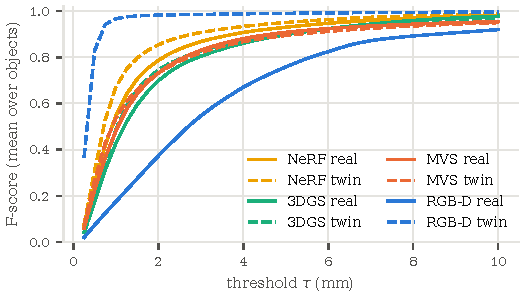
\includegraphics[width=\columnwidth]{figuras/fscore.pdf}
\caption{F-score versus threshold, averaged over the \nobj\ objects, for the real captures (solid) and their
digital twins (dashed).}
\label{fig:fscore}
\end{figure}

\subsection{Sim-to-real gap}
Fig.~\ref{fig:brecha} shows, for every object and method, the CD on the twin and on the real capture. For
the three image-based methods the twin is a good predictor of the real error: the mean gap is \nerfD~mm
for NeRF, \gsD~mm for 3DGS and \mvsD~mm for MVS (real-to-twin ratios of 1.0--1.2). Individual gaps stay
within $\pm 0.7$~mm, except for NeRF and 3DGS on the dark PETG part P1 ($+0.73$ and $+0.88$~mm) and 3DGS
on the translucent Caesar ($+0.72$~mm) (Table~\ref{tab:resultados}), where the real appearance is less favorable than the rendered one. The gap is
not always positive: 3DGS is less accurate on several twins than on the real captures (e.g., Bunny-L,
3.07 versus 2.49~mm), because its floaters depend on the rendered background and lighting, which are
approximations.

RGB-D fusion behaves differently: its mean real CD is ten times the twin value (gap \rgbdD~mm). The
per-method ICP explains most of this gap. Image-based clouds move only 0.1--1.3~mm (0.3--0.7~mm on average) when registered
individually to the CAD, i.e., they are consistent with the board frame defined by the ChArUco poses. The
RGB-D clouds move \rgbdshift~mm on average (2.5--6.4~mm for the opaque prints and 16.1~mm for Caesar), and
after this alignment the CD drops to 1.2--1.9~mm for the opaque objects, comparable to the image-based
methods. The dominant real RGB-D error is therefore a rigid offset between the L515 depth and the
photogrammetric frame, not the shape of the fused surface.

\begin{figure*}[!t]
\centering
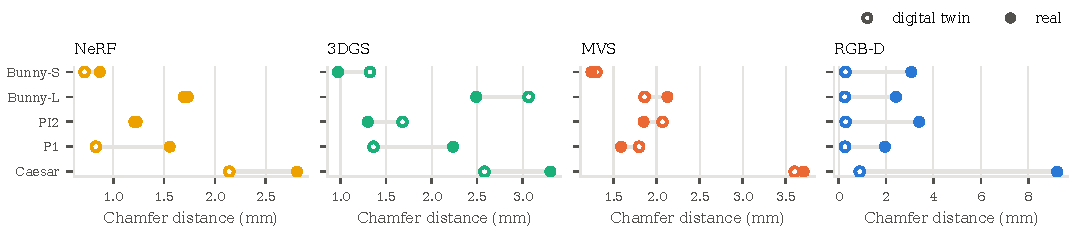
\includegraphics[width=\textwidth]{figuras/brecha.pdf}
\caption{Chamfer distance on the digital twin (hollow) and on the real capture (filled) for each object and
method. Note the different horizontal scales.}
\label{fig:brecha}
\end{figure*}

\subsection{Spatial distribution of the error}
Fig.~\ref{fig:error} shows the per-point error for the PI2 artifact. On both domains, the image-based
methods concentrate their error at concave features (the ring, the bores, the steps) and at the vertical
walls, where fewer views observe the surface; MVS additionally leaves gaps on low-texture surfaces. The
real RGB-D cloud exhibits an almost uniform error, the signature of a rigid offset, whereas its twin is
accurate everywhere.

\begin{figure*}[!t]
\centering
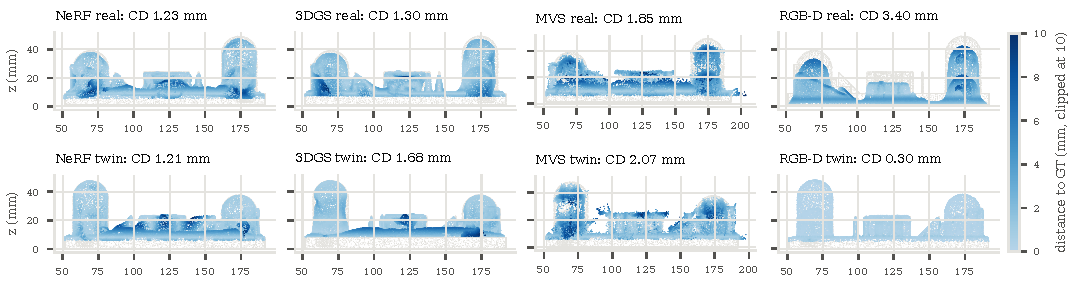
\includegraphics[width=\textwidth]{figuras/error.pdf}
\caption{Cleaned clouds of the PI2 artifact colored by distance to the CAD mesh (light gray), real capture
(top) and digital twin (bottom), side view.}
\label{fig:error}
\end{figure*}

\subsection{Effect of the material}
The translucent glow-in-the-dark PLA of Caesar is the hardest case for every method in both domains, but
especially for real RGB-D fusion: the near-infrared laser of the L515 penetrates the material, producing a
16~mm depth bias and a residual 9.0~mm CD even after ICP, an effect that the twin, which renders an opaque
material, cannot reproduce. The dark PETG of P1 increases the gap of the radiance-field methods (NeRF
$+0.73$~mm, 3DGS $+0.88$~mm) but not that of MVS ($-0.21$~mm).


% ============================================================================================
\section{Discussion}
\subsection{When is the twin a valid proxy?}
For passive, image-based reconstruction, the error budget is dominated by the reconstruction itself
(view coverage, texture, appearance), and the twin reproduces it: on average the real and simulated CD of
NeRF, 3DGS and MVS differ by $-0.02$ to $+0.32$~mm, with the same ranking in both domains. A twin with
calibrated cameras and replayed poses can therefore be used to select and tune these methods. For active
depth, the twin models the sensor as an ideal range measurement plus random noise, so it captures the
precision of the L515 but not its trueness: the depth-to-color extrinsics, a range bias that depends on the
material, and subsurface scattering are absent. The result is an optimistic prediction by a factor of ten.
Closing this gap requires a measured error model of the sensor (per-camera rigid bias and
material-dependent range bias), which the paired setup makes directly measurable: the per-method ICP
translation is an estimate of that bias.

\subsection{Uncertainty of the comparison}
Several error sources limit the resolution with which gaps can be resolved. The CAD-to-print deviation is
\printmae~mm MAE (max \printmax~mm). The ChArUco board poses have a median detector error of about 0.4~mm
in the twin, where the true pose is known, and the twin reproduces the board projections within 0.11~px.
The 4-DOF registration of the CAD to the real reconstructions has an RMS residual of about 1~mm on the
inlier points. Differences below roughly 0.5~mm between the real and simulated CD should therefore not be
interpreted as significant, which is the case for MVS and 3DGS on average.

\subsection{Choice of metric}
Accuracy, completeness and F-score lead to different conclusions than CD alone. On the real captures,
MVS has the best mean median accuracy of the image-based methods (0.86~mm versus 0.93~mm for NeRF) but a
worse completeness (1.34 versus 1.00~mm) and the largest H95 among them (10.8~mm), because it leaves
low-texture regions empty; its CD is therefore similar to that of 3DGS, whose clouds are complete but
thicker (median accuracy 1.22~mm). Reporting both directions of the distance and several thresholds is
necessary, in agreement with \cite{zielinski2026comparative,knapitsch2017tanks}.

\subsection{Limitations}
This study uses one capture per object, so the repeatability of the real measurements, and thus confidence
intervals of the gap, are not available. Materials and lighting of the twin were matched visually rather
than measured, the objects were not placed at their real pose on the board (the twin uses a canonical
placement, Section~\ref{sec:registro}), so the lighting direction relative to the object differs between
domains, the depth noise model is provisional, and the CAD-to-print deviation was measured with a
caliper on one artifact only. Color fidelity, which is relevant for the radiance-field methods, was not
evaluated. Finally, five objects and one trajectory do not cover the variability of textures,
reflectances and numbers of views that a full factorial study would require.


% ============================================================================================
\section{Conclusion}
We presented a paired benchmark that measures the sim-to-real gap of 3D reconstruction by reproducing each
real turntable capture of a 3D-printed object in a digital twin with identical camera calibration and
turntable poses, and by evaluating NeRF, 3DGS, MVS and RGB-D fusion with one protocol against the CAD model.
The twin reproduces fiducial detections within 0.11~px and silhouettes with IoU~$\geq$~0.975, and the
reference artifact deviates from its CAD by \printmae~mm on average. Over \nobj\ objects, the twin predicts
the accuracy of the image-based methods within a few tenths of a millimeter (mean gaps \nerfD, \gsD\ and
\mvsD~mm for NeRF, 3DGS and MVS), whereas it underestimates the real error of RGB-D fusion by an order of
magnitude because the real error is dominated by a 2.5--16~mm offset of the L515 depth with respect to the
photogrammetric frame, which is largest on a translucent material. Future work will incorporate a measured
sensor error model in the twin, repeated captures to obtain confidence intervals, swap experiments that
attribute the gap to poses, sensor and appearance, and color-fidelity metrics.


%\section*{Acknowledgment}
%\todo{Acknowledgments.}

\bibliographystyle{IEEEtran}
\bibliography{refs}

\end{document}
